\documentclass[a4paper, 11pt]{article}

\usepackage{amsmath}
\usepackage{amssymb}
\usepackage{titlesec}
\usepackage[utf8]{inputenc}
\usepackage[margin=1.5cm]{geometry}
\usepackage{prftree}
\usepackage{changepage}
\usepackage{enumitem}
\usepackage{minted}
\usepackage{lmodern}
\usepackage{graphicx}
\usepackage{wrapfig}
\usepackage{ulem}
\usepackage{marvosym}
\usepackage{xcolor}
\usepackage{mathtools}
\usepackage{bm}

\title{\vspace{-2cm}Mobile Sensor Systems\vspace{-1.5cm}}
\author{}
\date{}

\setlength{\parindent}{0cm}
\setlength{\parskip}{2mm}
\setlist{nosep}

% Make ~ look more normal
\let\oldsim\sim
\renewcommand{\sim}{{\oldsim}}

\newmintinline[monospace]{text}{escapeinside=\#\#, mathescape, fontsize=\normalsize}
\newminted[monospacefigure]{text}{frame=lines, framesep=1mm, autogobble, escapeinside=\#\#, mathescape, breaklines}

\titlespacing{\section}{0mm}{2mm}{2mm}
\titlespacing{\subsection}{0mm}{2mm}{2mm}
\titlespacing{\subsubsection}{0mm}{2mm}{2mm}

\begin{document}
\maketitle

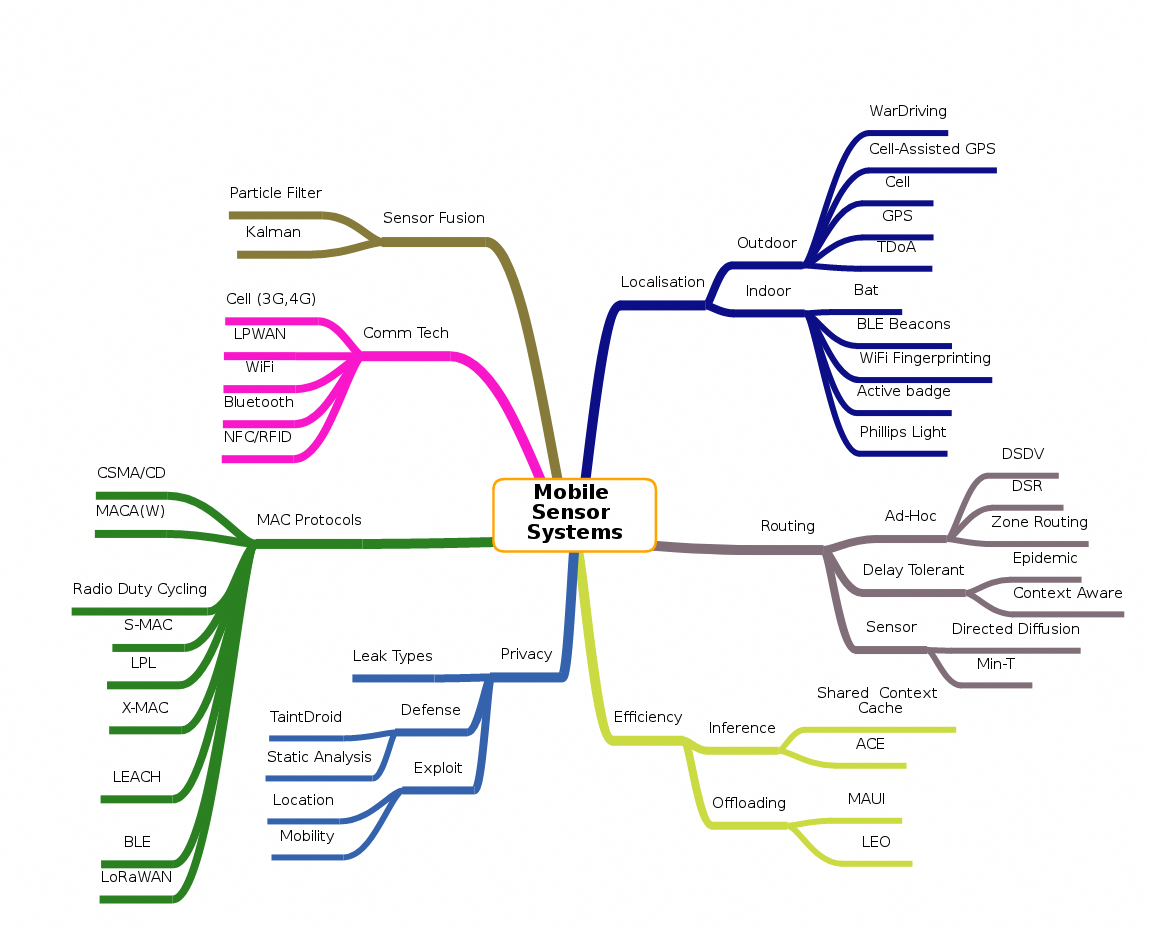
\includegraphics[angle=-90,width=\textwidth]{mindmap.png}
\newpage

\begin{itemize}
\item Proactive routing protocols maintain routes to nodes even when not being used -- usually expensive, but lower latency.
\item Reactive routing protocols find routes only when communication is needed -- comparatively high latency but cheaper for infrequent communication.
\item Reliable but long routes are better than short unreliable routes, for energy inefficiency. Using error correcting codes may add data and computation but reduce retransmissions.
\item Can't hurt to name-drop examples: when talking about inference, say `similar to in the ACE system'.
\item \textbf{On-device computation} is good for \textbf{privacy} -- don't send data to the cloud, keep it secure locally. Think of privacy issues.
\end{itemize}

\section*{Background}
{
    12 billion mobile devices -- almost everyone has phones, now sensors and IOT etc.\ is gaining traction.

    The internet is only available to most people through phones, no computers.

    Mobile data traffic is \(\approx\)0.5 \textbf{exabytes} per day.

    In the US, \(>\)50\% of internet access is through WiFi, rest is mostly 4G. In Nigeria 75\% is through 3G. Geographic areas have vastly different access patterns based on the infrastructure available and economics.

    Phones have a multitude of sensors:
    \begin{itemize}
    \item Camera
    \item Microphone
    \item Fingerprint
    \item Accelerometer
    \item Gyroscope
    \item Heart Rate
    \end{itemize}

    Mobile devices are resource- and energy-constrained. Connectivity is highly variable in \textbf{performance} and \textbf{reliability}. Mobile devices are inherently \textbf{less secure} (wireless communication means broadcast, which is snoopable).

    Types of connectivity, with energy/reliability/rate limits:
    \begin{itemize}
    \item Cellular (SMS, 3G, 4G, ...) -- large range.
    \item WiFi -- high energy cost on the receiver, but can have very high rates and quite high range.
    \item Bluetooth -- low cost (depends on protocol), low range.
    \item NFC -- very low range.
    \item Generic other radio communication
    \end{itemize}

    Wireless communication is generally organised as either:
    \begin{itemize}
    \item Infrastructure: Mobile devices connect to static base stations which are wired together into a trunk network. Handoff devices between base stations.
    \item Ad-hoc/Mesh: No base stations, devices communicate between themselves when they're in range or available. Node organise themselves into a network.
    \end{itemize}

    Medium (radio spectrum) is generally multiplexed between multiple devices:
    \begin{itemize}
    \item Time: fixed or dynamic.
    \item Frequency: each communication gets a disjoint frequency band.
    \end{itemize}

    Multiplexing as above doesn't scale well with lots of devices or if communication is sparse. Ad-hoc approaches allow more statistical multiplexing:
    \begin{itemize}
    \item
    {
        CSMA/CD: transmit if nothing else is, jam if you detect a collision, randomised binary exponential backoff.

        \begin{minipage}[t]{0.65\textwidth}
        \setlength{\parskip}{8pt}
        \begin{itemize}
        \item Hidden Terminal: if \(A\) transmits to \(B\), any data \(C\) sends will cause a collision, but \(C\) can't tell that \(A\) is sending.
        \item Exposed Terminal: if \(B\) transmits to \(A\), \(C\) can't transmit in case it causes a collision at \(A\), but \(A\) is out of range of \(C\).
        \end{itemize}
        \end{minipage}
        \hspace{3mm}
        \begin{minipage}[t]{0.25\textwidth}
        \vspace{2mm}
        \centering
        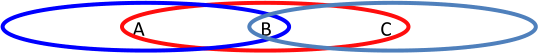
\includegraphics[width=\textwidth]{terminals.png}
        \end{minipage}
    }
    \item
    {
        Multiple Access with Collision Avoidance for Wireless (\textbf{MACAW}): Sender sends an RTS, receiver signals CTS if available. Potential interferers see the transmissions and know whether to wait or request from the combinations of packets (eg.\ see a RTS but no CTS within a timeout, the requester is probably hidden).
    }
    \end{itemize}

    Some powered devices have a maximum current draw -- need to control which subdevices are active at each time to prevent overloading (eg.\ can't run radio and process data at the same time).
}
\section*{Ad-Hoc Networks}
{
    Defining feature is that there's no existing infrastructure: the network configures itself dynamically. Uses in:
    \begin{itemize}
    \item Rescue operations.
    \item Military operations.
    \item Autonomous vehicles.
    \end{itemize}

    These routing protocols assume that there's a \textbf{complete route between source and destination at the same time}.

    \subsection*{Destination Sequenced Distance-Vector Routing}
    {
        Distance-vector style protocol. Each node maintains a table indexed by destination node containing: \textbf{next hop}, \textbf{hops required}, and \textbf{sequence number}. Each node also carries a randomly-initialised counter used for generating the sequence numbers for transmissions from it. Sequence numbers represent recentness of data.

        Every node periodically transmits its full routing table to ensure convergence throughout the network, but also sends smaller incremental updates frequently.

        When a node becomes aware of multiple routes to the same node, it picks the route with the \textbf{greatest sequence number}, which \textbf{avoids loops} and ensures we use the most recent route.

        \begin{itemize}
        \item When a node joins the network, it transmits its \textbf{sequence number incremented by 2}, and the \textbf{full routing table} (either a single entry to itself if it's a sole node, or a full table if it's part of a disjoint subnet). Nodes within range update their table with the new node's table, then propagate the relevant changes to neighbours (incremental update).
        \item When a node leaves the network, each node notices the break (eg.\ no table update within a timeout), so updates the hop count to that node to \(\infty\) and \textbf{increments the sequence number}, then propagates the changes to neighbours.
        \end{itemize}

        Incrementing the sequence number on a disconnect is to force the other tables to use the new routing information, as the sequence number is higher than the old one. When we see an update from the destination node, it'll have sequence number of 2 more than the original, which makes it more recent.

        The incremental changes essentially flow recursively throughout the graph, with nodes updating their tables and recursively propagating any changes.

        Proactive protocol, and is generally wasteful of energy.
    }
    \subsection*{Dynamic Source Routing}
    {
        Style of flood routing, but we only flood route requests rather than the data -- less data, and we can cache the route taken.

        When a node needs to communicate it sends a packet to its neighbours requesting a route to the destination. Nodes receive the packet, add themselves to the route stored inside it, and propagate to their neighbours.

        When the packet reaches the destination, it sends a confirmation back to the source along the reverse path in the packet, and the source transmits the data.

        If links are non-symmetric, then the destination might need to send a route request for A as it can't just use the reverse path.

        Use sequence numbers on packets to avoid routing loops, and nodes can cache the partial routes they see in packets to reduce the number of route requests.
    }
    \subsection*{Zone Routing Protocol}
    {
        Combines reactive and proactive approaches: each node proactively maintains routes in a zone around itself, then an inter-zone protocol is used to reactively determine routes between the zones.
    }
}
\section*{Delay-Tolerant Networks}
{
    Ad-hoc networks where there's \textbf{not necessarily a complete path from source to destination at the same time}. Nodes can accept a packet and deliver it later.

    \subsection*{Epidemic Routing}
    {
        Flood protocol which allows nodes to store packets before forwarding.

        Packets are passed to a configurable fraction of neighbours of each node, which store it for a while. As nodes travel and meet new neighbours, they forward the message and \textbf{stop remembering it} after a while.

        Needs large buffers on nodes, and the forwarding number needs tuning to avoid network transmissions and collisions.
    }
    \subsection*{Context Aware Routing}
    {
        Improvement to epidemic routing: instead of blindly forwarding to neighbours, nodes present information about their mobility and commonly-visited neighbourhoods, and maybe even allow preferences as to their route.

        Based on the exposed metrics, transmitting nodes pick neighbours which have the best chance of reaching the destination, or maybe delay sending until there's more choice.

        Combine the following metrics with a utility function:
        \begin{itemize}
        \item Mobility (how much/often the node moves).
        \item Host colocation with destination (use a Kalman filter to predict future host colocation based on prevous colocation).
        \item Energy budget.
        \end{itemize}
    }
}
\section*{Mobile Sensor Networks}
{
    Sensor networks produce far more data far more easily than traditional manual monitoring. Usually have a large number of low-unit-cost battery-powered wireless devices.

    \begin{itemize}
    \item Structural health monitoring (humidity, stress, vibrations, ...).
    \item Environmental monitoring (air quality, noise pollution, ...).
    \item Animal behaviour.
    \item Warehouse logistics.
    \end{itemize}

    Can use ad-hoc networks between sensors, with a few static gateways on the edge to link the network to the internet.

    Differences from mobile sensor systems:
    \begin{itemize}
    \item Sensor nodes are prone to failure, as they're often deployed in harsh conditions.
    \item Higher numbers of nodes, so each unit is cheaper and more resource constrained than a mobile node.
    \item Usually a relatively static layout -- sensor nodes don't usually move, or only a subset do.
    \end{itemize}

    \subsection*{Energy Consumption}
    {
        Local computation is cheap -- running the processor, keeping stuff in RAM, sampling sensors is all inexpensive. \textbf{The \textit{radio} is the main energy sink}. \textbf{Idle listening is as expensive as transmitting}, so the cost is on the receiver.

        To improve power efficiency, want to switch off the radio on sensors \textbf{instead of leaving it idle}.
    }
    \subsection*{Radio Duty Cycling}
    {
        Use a global clock across sensors to have them all only activate radios at a specific time, and spend the rest of the time turned off. Requires precise synchronisation or the sensors remain idle for too long.
    }
    \subsection*{Sensor-MAC (S-MAC)}
    {
        \textbf{Synchronised protocol}: negotiates a communication schedule among neighbouring nodes. Each node has a specific \textbf{wakeup} schedule that determines when it idly activates the antenna.

        Every node knows each neighbour's wakeup schedule.

        3 phases during each activation:
        \begin{enumerate}
        \item SYNC: Use CSMA to tell neighbour nodes about the node's wakeup schedule.
        \item RTS: Listen for RTS packets, if we receive one then run the CTS stage -- otherwise go back to sleep after the period.
        \item CTS: Send a CTS to the requesting node, extend the wakeup time so we can receive the data.
        \end{enumerate}

        When a node wants to transmit to a destination, it sleeps until the next active time in the \textbf{destination's schedule} and then sends a RTS.

        New nodes try to pick up an existing wake schedule, rather than make their own one. If a node learns of two different schedules, we end up with \textbf{synchronised islands} -- the node has to follow \textbf{both wakeup schemes} so wastes more energy.
    }
    \subsection*{Low Power Listening (LPL)}
    {
        \textbf{Asynchronous protocol}: relies on \textbf{preambles} to connect a transmitter to the relevant receivers.

        Receivers sleep and only periodically sample the channel. Senders prefix the message with a long transmission of meaningless data, so that when a receiver wakes up it notices that there's something about to be sent and stays awake to see what it is.

        Issues:
        \begin{itemize}
        \item Overhearing: All receivers listening to the preamble have to stay awake to hear who the intended receiver is.
        \item Long preamble wastes energy in transmission and for receivers who stay awake until it's over.
        \item Latency introduced by the additional information.
        \end{itemize}
    }
    \subsection*{X-MAC}
    {
        \begin{minipage}[t]{0.55\textwidth}
        Improvement on LPL:
        \begin{itemize}
        \item Use multiple shorter preambles (shorter summed length than a long preamble).
        \item Include target address information in the preamble so receivers can tell if it's for them or not.
        \item
        {
            When a receiver notices a preamble:
            \begin{itemize}
            \item If they're not the target receiver, they go back to sleep.
            \item Otherwise, they send an ack signal to the transmitter, which terminates the preamble early and allows for immediate communication.
            \end{itemize}
        }
        \end{itemize}

        Significant improvement on energy and time cost, and not much more complicated.
        \end{minipage}
        \hspace{3mm}
        \begin{minipage}[t]{0.4\textwidth}
        \vspace{0pt}
        \centering
        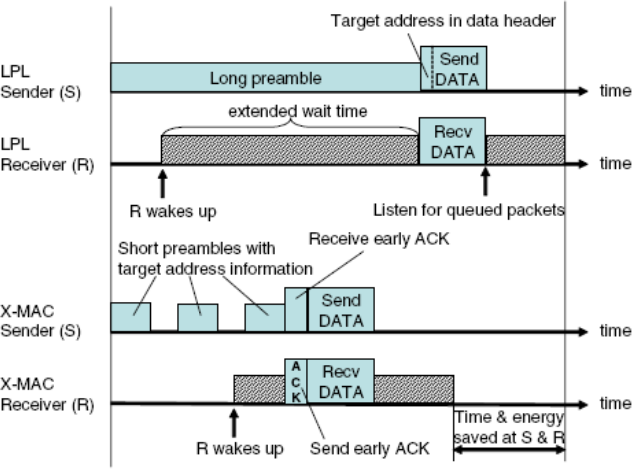
\includegraphics[width=\textwidth]{xmac.png}
        \end{minipage}
    }
    \subsection*{Low-Energy Adaptive Clustering Hierarchy (LEACH)}
    {
        Group nodes into clusters controlled by a clusterhead. Nodes talk to the clusterhead cheaply, clusterhead talks to the centralised data sink.

        Aim is to offload expensive communication onto a subset of nodes, and transfer responsibility frequently to prevent nodes dying quickly. Non-clusterhead nodes can communicate cheaply using TDMA (only transmit if they need to, so no wasted energy on normal nodes). Clusterheads drain power quickly as they have to be idly receiving constantly.

        \textbf{Assumptions}:
        \begin{itemize}
        \item \textbf{Dense network of nodes}
        \item \textbf{Nodes report to a clusterhead}
        \item \textbf{All nodes in a cluster can communicate with the clusterhead directly}
        \item \textbf{Clusterheads can reach a central sink in one hop}
        \end{itemize}

        \begin{enumerate}
        \item
        {
            Setup:
            \begin{enumerate}
            \item Clusterheads elect themselves based on a probability for each node (and not being a clusterhead too frequently).
            \item Nodes join the nearby clusterhead with the strongest signal.
            \item Clusterheads organise CDMA between heads, and set up TDMA between nodes within a cluster.
            \end{enumerate}
        }
        \item Steady State: Clusterheads collect and \textbf{aggregate} data from cluster members, then transmit it to the central sink using CSMA. Aggregation can be as simple as concatenating packets -- still reduces overhead so is more efficient.
        \item Each `\textbf{round}' of LEACH is a fixed duration, after which clusterheads are selected again and the process repeats.
        \end{enumerate}
    }
}
\section*{Internet of Things}
{
    \begin{minipage}[t]{0.65\textwidth}
    \setlength{\parskip}{8pt}
    Extend internet connectivity into everyday things -- embed internet-capable devices into things. Allows for metrics and data and remote control.

    Scopes:
    \begin{itemize}
    \item Devices: sensor nodes, mobile phones, wearable gear, ....
    \item Machines: home appliances, vehicles, security systems, ....
    \item Environments: smart homes, buildings, cities, ....
    \end{itemize}

    Typical Architecture:
    \begin{itemize}
    \item Device: basic processing, short communications. Perform sensing and/or actuation.
    \item Gateway: edge analytics and local storage, routing.
    \item Cloud: service hosting, visualisation, advanced analytics, long-term data storage.
    \end{itemize}
    \end{minipage}
    \hspace{3mm}
    \begin{minipage}[t]{0.3\textwidth}
    \vspace{0pt}
    \centering
    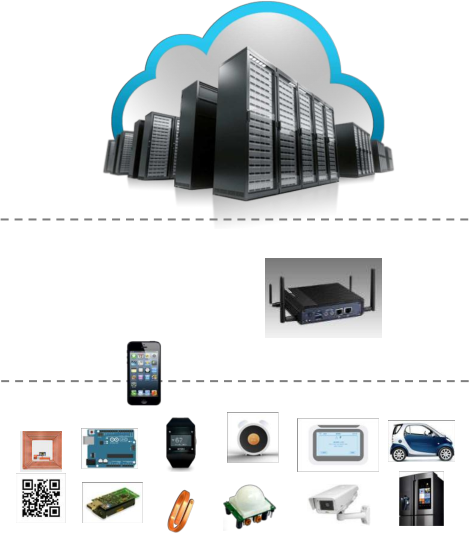
\includegraphics[width=\textwidth]{iot.png}
    \end{minipage}
}
\section*{Communication Technologies}
{
    \begin{center}
    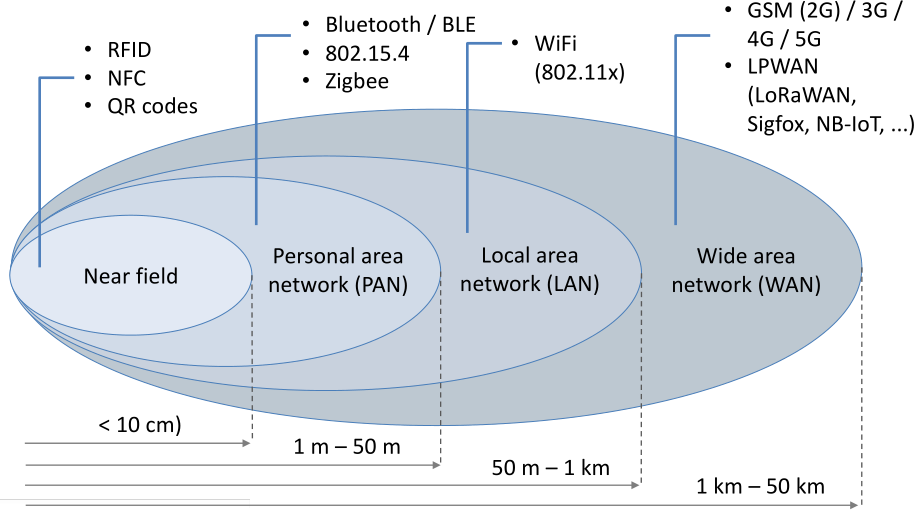
\includegraphics[width=0.5\textwidth]{commtech1.png}
    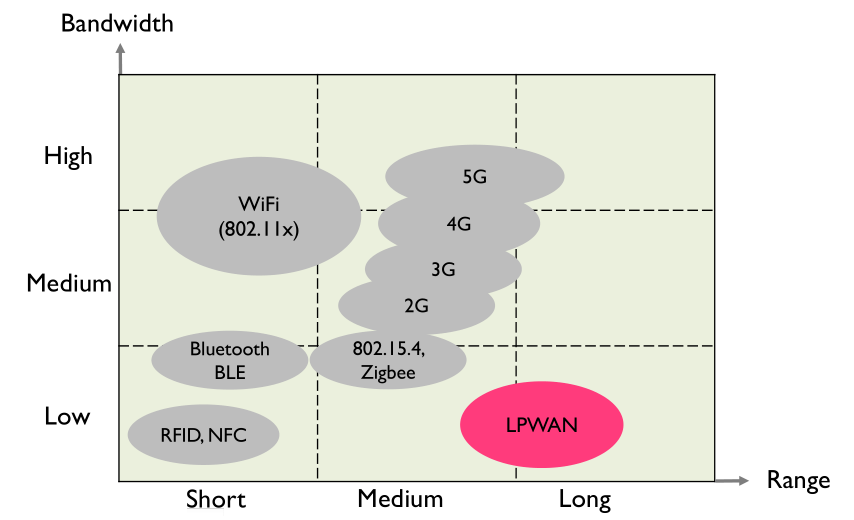
\includegraphics[width=0.45\textwidth]{commtech2.png}
    \end{center}

    \textbf{Low Power Wide Area Networks} (\textbf{LPWANs}) are an outlier in the existing communication technologies, and are what IoT and mobile devices need:
    \begin{itemize}
    \item Large ranges.
    \item Very small bandwidth requirements.
    \item Low power.
    \item Deep indoor penetration.
    \item Cheap and small radio modules.
    \item Usually relatively \textbf{delay tolerant} -- maybe only transmit a few packets each hour.
    \end{itemize}

    \textbf{LoRaWAN} is a protocol for LPWAN applications. Covers three types of end-device classes:
    \begin{description}
    \item[Class A]
    {\hfill
        \begin{itemize}
        \item Battery powered
        \item Bidirectional communication
        \item Initiates communication, isn't contacted by a remote
        \item Low power consumption, but high latency
        \end{itemize}
    }
    \item[Class B]
    {\hfill
        \begin{itemize}
        \item Battery powered
        \item Same as Class A but has more receive windows -- used for eg.\ edge devices and routers
        \item High power consumption, low latency
        \end{itemize}
    }
    \item[Class C]
    {\hfill
        \begin{itemize}
        \item Mains-powered
        \item Constantly receiving, base station equivalent
        \item High power consumption, low latency
        \end{itemize}
    }
    \end{description}
}
\section*{Sensor Network Routing}
{
    Routing specifically in networks of sensors -- aims are different, it's less commonly communication and more just data reporting to a single sink/data fetching by a single requester.

    Specific nodes are interested in specific events -- a sink is interested in a sensor's reading changing.

    Can still use ad-hoc networks like epidemic, DSDV, but there's an overhead from the general-purpose design. Additionally, they're more usually built for disconnections/delay tolerance, whereas sensor networks are normally static.

    Want \textbf{pub/sub} control, with a device subscribing to a type of data and then receiving relevant messages.

    \subsection*{Aggregation}
    {
        Quick diversion -- sending fewer packets saves energy, so particularly in sensor networks, may want to combine data:
        \begin{itemize}
        \item Average/min/max of readings.
        \item Compress results.
        \item Minor pre-processing on-device, rather than doing it all at the destination.
        \end{itemize}
    }
    \subsection*{Directed Diffusion}
    {
        Nodes send `\textbf{interests}' for data which get diffused through the network -- sensor data is tagged with interests and routed.

        Each node remembers which neighbours had which interests (propagated recursively). Interests have a `rate of events', called `\textbf{gradient}' -- sensor data sources emit events to neighbours which have a gradient for the data's interest at a \textbf{rate proportional to the interest gradient}: a higher gradient results in more events being sent.

        Event IDs are stored to avoid cycles (check event hasn't been received before).

        When gradients are established the rate is defined as a low default value. Sinks `reinforce' good paths, which results in a greater gradient and higher rate.

        Paths expire after a timeout so if not reinforced, they cease to exist. This allows for adaptation in the network.

        \textbf{Intermediate or sink nodes which receive duplicate data can choose to not reinforce the gradient on a redundant link} -- this allows nodes to control the paths used by data, and with a good utility function causes the interest paths to naturally converge to good routes.

        \subsubsection*{Extensions}
        {
            Push diffusion: if there are more receivers than senders, it's more efficient to flood the data rather than interests -- can still use gradients, but they're for data rather than interests.
        }
        \subsubsection*{Issues}
        {
            No consideration of link stability or link load.

            MAC layer issues -- assumes that nodes are listening all the time.
        }
    }
    \subsection*{MinT Routing}
    {
        Number of hops isn't necessarily a good metric in sensor networks -- reliability has a big impact on energy efficiency as retransmissions are expensive.

        MinT routing is distance-vector but using an estimation of the cost of retransmitting over the whole route, using relatively realistic link cost estimates.
    }
}
\section*{Mobile and Wearable Sensors}
{
    General-purpose sensors with a general-purpose multi-tasking OS, well-suited for human activities and easily maintainable (easy to update, user recharges device). Contrast to mobile sensor systems, which are made for measuring specific phenomena in a specific environment, with all resources dedicated to that.

    \textbf{Human Activity Detection}: accelerometer or gyroscope, used to infer eg.\ walking/running/cycling. Used for fitness monitoring.
    
    \textbf{Transportation Mode Detection}: accel and gyro, but also GPS and WiFi localisation, to infer bus, bike, car, etc. Used for smart commuting, data-driven transport network decisions.

    \textbf{Emotion Detection}: microphone, location data. Maps speaking features to emotional state -- used for social science experiments and behaviour intervention.

    \textbf{Context and Environment}: microphone, camera. Infers the social activity, used for health and wellness or eg.\ automated diary.

    Broad issues: heterogeneity of sensors reduce generalisation of techniques due to sensitivity/power/frequency differences. Privacy issues are big, measurements are noisy, and there's limited processing/battery power.
}
\section*{Energy Efficiency in Inference}
{
    Continuous monitoring is constantly polling sensors -- very expensive in general, but `required' to trigger actions.

    Use duty cycling on sensors, to only enable them for windows of time. Downside is that the view of user activity is incomplete in the downtime.

    \subsection*{Shared Context Sensing}
    {
        Use a shared cache of sensor output, maybe also cache inferences made such as \texttt{Driving?}. When an app requests a value, we poll the sensor/infer the value then cache it. A different app requesting the same data later gets a cached value rather than recomputing.
    }
    \subsection*{ACE}
    {
        Can infer some features from other features -- if an app requests the value of \texttt{AtHome} we can infer the value from the negatively-correlated \texttt{Driving} feature, which we've had cached. Means we avoid polling GPS and WiFi localisation data.

        Builds on the shared cache, as we want to reuse data between apps.

        Usually want the cheapest method of inferring a feature, so use eg.\ \texttt{Running} to infer the value of \texttt{AtOffice} instead of using \texttt{AtHome}, as \texttt{AtHome} may be expensive compared to the accelerometer check.

        \textbf{Rule Miner}: automatically learns relationships between various features by looking for positive or neagative correlation.

        \textbf{Sensing Planner}: finds a cheap sequence of proxy sensors to sample in order to determine a target feature. Heuristics manually added to make the problem tractable.

        \textbf{Inference Cache}: return a cached value if it exists, or infer the value using the sensing planner if possible. If not, directly poll the sensor and cache.
    }
    \subsection*{MAUI}
    {
        Offloading data to the cloud can be wasteful, given the high cost of transmitting and the power of current mobile devices. Eg.\ using an on-chip GPU for updating a model can be massively faster and less expensive than uploading all the data to the cloud for processing then downloading the updated model. This is especially true on unreliable networks.

        MAUI profiles code components to determine whether they should be run locally or remotely, taking into account:
        \begin{itemize}
        \item Cost of transferring code/data.
        \item Latency.
        \item Network constraints.
        \end{itemize}

        However, it only considers the CPU -- there are dedicate GPUs, DSP units, even some machine learning FUs on movile devices.
    }
    \subsection*{LEO}
    {
        Improvement to MAUI which has profiles for different on-chip resources, and can dispatch execution to any of them or the cloud.

        Very good for continuous audio sensing, as we can use on-chip DSP processors instead of transmitting the audio stream.
    }
}
\section*{Privacy}
{
    Lots of user generated data, permission control is still quite coarse -- apps can generate data for advertising use, but there's no system-level verifiable control of where the data can go, it's all in the contract/terms-of-usage.

    \subsection*{TaintDroid}
    {
        Android variant that allows for tracking sensitive data movement in and between apps at runtime. Labels data from privacy-sensitive sources (most sensors, some system information/preferences) and propagates labels as the data propagates through variables, files, and IPC.

        When tainted data leaves the system (transmitted, saved to an external device, ...), TaintDroid logs the data labels, the application responsible for the transmission, and the data destination.

        Runtime, so relatively easy to `just run', but imposes a runtime performance hit.
    }
    \subsection*{Static Analysis}
    {
        Statically verify all the paths from sources to sinks within an app/system.

        Much much much more effort than dynamic analysis, but no runtime efficiency overhead.
    }
    \subsection*{Cell Network Leaks}
    {
        Mobile devices roam around and register with base-stations -- data leaks from the station records can uniquely identify users.

        Some cell protocols can be directly vulnerable to locational attacks due to broadcasting.
    }
    \subsection*{WiFi Leaks}
    {
        WiFi device id or MAC addresses are broadcast -- extra vulnerable on open WLANs. Information freely broadcast is enough to track locations of devices across networks.

        Specific personally-identifying information can be gained from applications, websites, ad content, traffic data in WiFi hotspots -- open WiFi is death.
    }
    \subsection*{Mobile Sensor Leaks}
    {
        Accelerometers are different on all devices -- can be used as a per-device signature or fingerprint, or used to identify different users of the same device. Touch sensor usage, keyboard patterns, .... 
        
        Even in anonymised datasets, identifying a specific user is relatively easy given activity profiles. Correlation of activities introduces information.
    }
    \subsection*{Mobility Prediction}
    {
        Given past mobility information, can infer future mobility. Even more effective when combined with friends/family/coworker information.

        Colocating in both time and space is hard, but shown to be possible and demonstrated.
    }
}
\section*{Localisation}
{
    With eg.\ WiFi/GPS positioning, we measure the \textbf{time-of-flight} (ToF) of signals from various base-stations with known position to the receiver, then use trilateration to place the device.

    Reflections of signals are fine for communication, but make positioning way harder -- indoors is significantly harder than outdoors. Outdoors is still hard, as a difference of 1\(\mu\)s is 300m.

    \subsection*{Timed Difference of Arrival (TDoA)}
    {
        Sync all the static clocks (lay wire between them, or use atomic clocks). The device transmits a signal at time \(t_p\), and static stations detect at times \(t_A,t_B,t_C\). Then:
        \begin{gather*}
        c(t_A - t_p) = d_{AP}
        \qquad
        c(t_B - t_p) = d_{BP}
        \\
        c(t_A - t_C) = d_{AP} - d_{BP}
        \end{gather*}

        The 3 equations define 3 hyperbolas, and their intersection is the transmitter location.
    }
    \subsection*{GPS}
    {
        TDoA system but the satellites are both the `static' devices and the transmitters. Each satellite sends the time at the satellite, and the device finds the relative local clock skew. After multiple readings from GPS, have equations for location.
    }
    \subsection*{Cellular Localisation}
    {
        Cell towers give coarse proximity for devices connected to it (varying ranges depending on eg.\ rural vs urban base-station).

        Use TDoA with the base-stations, base-stations use GPS to sync.
    }
    \subsection*{Wardriving}
    {
        WiFi fingerprinting on a large scale -- build up national maps of WiFi networks using GPS location and a WiFi receiver, can then get \(\approx\)50m accuracy on devices just by seeing what networks are available.
    }
    \subsection*{Angle of Arrival (AoA)}
    {
        Use multiple antenna positioned slightly apart to detect time differences in reception, and infer the angle of the transmitter.

        Still has issues with reflection/multipath, but gives direction information rather than radius information.
    }
    \subsection*{Indoor Location}
    {
        GPS fails -- it can't penetrate or gets reflected, and even if we had accurate measurements of eg.\ 3m, that's too large scale for indoor use.

        \subsubsection*{Active Badge}
        {
            Original microlocation device -- room-scale location by transmitting an ID using infrared, with sensors in rooms detecting the IDs.
        }
        \subsubsection*{BLE Beacons}
        {
            Beacon range of 1-3m, can position around an indoor environment and use a database of beacon positions for coarse positioning.
        }
        \subsubsection*{Phillips Lights}
        {
            Lights flicker faster than we can see, then phone cameras decode the flicker sequences into room IDs.
        }
        \subsubsection*{Bat System}
        {
            TDoA where the device transmits to a network of receivers in the roof, connected in a mesh.

            Uses \textbf{ultrasound}, which is slower so more easily measurable than radio. Can get 3cm accuracy.

            Ultrasound has low penetration, which contains it inside a room but also means the device effectively needs line-of-sight to ceiling sensors. It's also disturbing to animals, and easy to disrupt.
        }
        \subsubsection*{WiFi Fingerprinting}
        {
            Perform a manual mapping of the signals available and their strengths at points in an environment.

            Devices measure signals when moving and finds the closest matching recorded location.

            Issues when APs die or are moved. Can give every non-present AP a baseline strength (eg.\ lowest possible reception strength), so that comparisons are more balanced, but every approach has nasty corner cases.
        }
        \subsubsection*{Particle Filters}
        {
            Essentially a general particle filter using accelerometer for sensor input and domain-specific model being a floorplan and discarding particles that pass through walls.
        }
    }
}
\section*{Sensor Fusion}
{
    Sensor measurements are noisy, error creeps in whatever we do.

    Idea is to estimate a true value using:
    \begin{itemize}
    \item Multiple measurements from the same sensor.
    \item Multiple measurements from different sensors.
    \item A domain-specific model of the constraints.
    \end{itemize}

    \textbf{Filters} estimate current state based on past and current measurements (live processing).

    \textbf{Smoothers} are post-processing, they use past, current, and future measurements to `smooth' the data.

    \subsection*{Kalman Filter}
    {
        Write the rules of the system with linear algebra (current state as a vector, motion model as a linear transform, ...). Introduce error to each term.

        \begin{enumerate}
        \item Start with an estimate of the initial position as a Gaussian representing the belief of that state.
        \item Update the estimate with the motion model to form a predition.
        \item Perform a measurement to get a noisy reading of the current measurement.
        \item Multiply the two Gaussian distributions together to get an updated prediction.
        \end{enumerate}

        Very fast, very accurate with good initial state, used everywhere.

        If the probability distributions aren't really Gaussian, can be inaccurate (need domain-specific info to encode eg.\ a floorplan).
    }
    \subsection*{Particle Filter}
    {
        Encode state in particles within a state space:
        \begin{enumerate}
        \item \textbf{Propagate} (new predictions): In the floorplan example, move them in the encoded direction by a step length.
        \item \textbf{Correct}: reassign the probabilities of the particles, our belief that they're correct. In the floorplan example, particles passing through a wall would be corrected to 0 probability.
        \item \textbf{Resample}: Generate a new set of particles by sampling the old one in proportion to the weights of the particles. Low probability particles are less likely to have new particles near them.
        \end{enumerate}

        Allows starting with no knowledge of initial state.

        Two general phases:
        \begin{itemize}
        \item \textbf{Localisation} uses lots of particles to find the current state is from an unknown initial state. 
        \item \textbf{Tracking} uses fewer particles once we've found the state to improve efficiency.
        \end{itemize}
    }
}
\section*{Bluetooth Low Energy}
{
    Classical bluetooth is for replacing wires with wireless. BLE is for enabling new applications.

    \textbf{2 main modes}:
    \begin{itemize}
    \item Advertise: Nodes broadcast eg.\ sensor information -- other nodes in range receive it if they want.
    \item Connection: Masters can connect to slave nodes, which are found through advertising -- presumably just advertise as `connectable' and other nodes can directly connect.
    \end{itemize}

    Seems to be useful for application level, if we want broadcast communication it's easy, if we want connection then we just piggyback discovery on the existing service.

    Technically a MAC protocol, it's below network layer.
}
\section*{Robots}
{
    \begin{description}
    \item[Proprioceptive Sensors]: `body' sensors like motor speed, battery voltage, joint angle.
    \item[Exteroceptive]: `environment' sensors like distance measurement, light intensity.
    \item[Passive]: `measure ambient energy' like thermometers, microphones.
    \item[Active]: `emit energy' like infrared/ultrasound proximity sensors.
    \end{description}

    \textbf{Coverage} aims to deploy sensors over an area in different ways:
    \begin{description}
    \item[Blanket]: \textbf{Static arrangement} to \textbf{cover} an area.
    \item[Barrier]: \textbf{Static arrangement} to minimise the probability of undetected penetration of the barrier.
    \item[Sweep]: \textbf{Move sensors} across an area to maximise the number of detections and minimise missed detections.
    \end{description}

    \textbf{Voronoi Coverage} defines families of blanket coverage styles that optimise the configuration of robots.

    \textbf{Centroidal Voronoi Tessellation} (CVT): minimises the average distance between robots and all points in their cells -- optimal blanket arrangement.
}
\end{document}